\documentclass[12pt,a4paper,onecolumn]{article}

%%%%%%%%%%%%%%%%%%%%%%%%%%%%%%%%%%%
% PAQUETES
%%%%%%%%%%%%%%%%%%%%%%%%%%%%%%%%%%%

\usepackage[margin=1in]{geometry}
\usepackage{authblk}
\usepackage[utf8]{inputenc}  % UTF-8 evita problemas de caracteres
\usepackage[T1]{fontenc}     % Mejor soporte de fuentes en LaTeX
\usepackage[spanish]{babel}  % Manejo correcto de idioma español
\usepackage{amsfonts}
\usepackage{graphicx} % Necesario para incluir imágenes
\usepackage{xcolor}
\usepackage{amsmath}
\usepackage{amssymb}
\usepackage[table]{xcolor}
\usepackage{setspace}
\usepackage{booktabs}
\usepackage{dcolumn}
\usepackage{rotating}
\usepackage{threeparttable}
\usepackage[capposition=top]{floatrow}
\usepackage[labelsep=period]{caption}
\usepackage{subcaption}
\usepackage{multicol}
\usepackage[bottom]{footmisc}
\usepackage{enumerate}
\usepackage{units}
\usepackage{placeins}
\usepackage{booktabs,multirow}
\usepackage{booktabs} % Para tablas mejoradas

% Bibliografía
\usepackage{natbib}
\bibliographystyle{apalike}
\bibpunct{(}{)}{,}{a}{,}{,}

% Formato de párrafos
\renewcommand{\baselinestretch}{1}

% Definir columnas para tablas
\usepackage{array}
\newcolumntype{L}[1]{>{\raggedright\let\newline\\\arraybackslash\hspace{0pt}}m{#1}}
\newcolumntype{C}[1]{>{\centering\let\newline\\\arraybackslash\hspace{0pt}}m{#1}}
\newcolumntype{R}[1]{>{\raggedleft\let\newline\\\arraybackslash\hspace{0pt}}m{#1}}

\usepackage{xfrac}
\usepackage{bbold}

\setcounter{secnumdepth}{6}

\usepackage{titlesec}
\titleformat*{\subsection}{\normalsize \bfseries}

\usepackage[colorlinks=true,linkcolor=black,urlcolor=blue,citecolor=blue]{hyperref}

%%%%%%%%%%%%%%%%%%%%%%%%%%%%%%%%%%%
%     TÍTULO, AUTORES Y FECHA              %
%%%%%%%%%%%%%%%%%%%%%%%%%%%%%%%%%%%

\title{\textbf{Taller 2 - Predicción de Pobreza en Colombia}}

\author{%
\begin{center}
Harold Stiven Acuña\\
José David Cuervo\\
José David Dávila\\
César Augusto Alfaro
\end{center}%
}

\date{\today}

% Configuración simple para espaciado de párrafos
\setlength{\parskip}{0.6em} % Espacio entre párrafos
\setlength{\parindent}{1em} % Sangría moderada

\begin{document}

\maketitle
\thispagestyle{empty}

%%%%%%%%%%%%%%%%%%%%%%%%%%%%%%%%%%%
% ABSTRACT
%%%%%%%%%%%%%%%%%%%%%%%%%%%%%%%%%%%

\begin{abstract}
Este documento presenta el análisis de datos y la implementación de modelos de clasificación para la predicción de la pobreza en Colombia.
\end{abstract}

\medskip

\begin{flushleft}
    {\bf Palabras clave:} pobreza, clasificación, aprendizaje automático \\
    {\bf Clasificación JEL:} J31, C53, J16
\end{flushleft}

% Añadir información del repositorio GitHub
\begin{center}
    \textit{Repositorio GitHub:} \url{https://github.com/alfarocesar/BDML_Predicting_Poverty_Equipo8}
\end{center}

\pagebreak
\doublespacing

%%%%%%%%%%%%%%%%%%%%%%%%%%%%%%%%%%%
%           DOCUMENTO                       %
%%%%%%%%%%%%%%%%%%%%%%%%%%%%%%%%%%%

\section{Introducción}
Breve descripción del problema, antecedentes y motivación del estudio.

\section{Datos}
\subsection{Descripción de la base de datos}
Explicación de la estructura de los datos y variables clave.

\subsection{Procesamiento y limpieza de datos}
Metodologías aplicadas para la adecuación de los datos.

\subsection{Análisis descriptivo}
Exploración de la variabilidad de los datos con tablas y gráficos.

% Este es un ejemplo de como incorporar las gráficas en el documento
\begin{figure}[htbp]
    \centering
    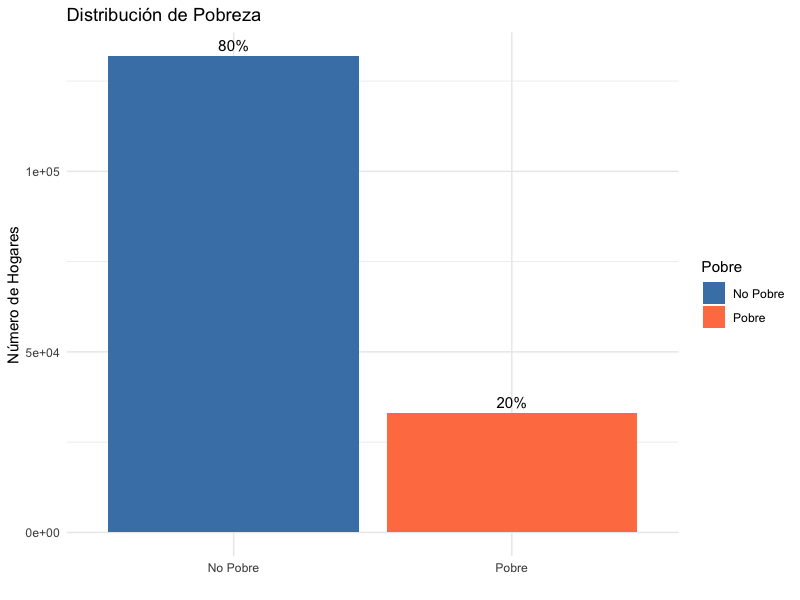
\includegraphics[width=0.8\textwidth]{../views/figures/poverty_distribution.png}
    \caption{Distribución de la pobreza}
    \label{fig:distribución_pobreza}
\end{figure}

% Este es un ejemplo de como incorporar tablas en el documento

% Table created by stargazer v.5.2.3 by Marek Hlavac, Social Policy Institute. E-mail: marek.hlavac at gmail.com
% Date and time: Mon, Mar 31, 2025 - 11:02:03
\begin{table}[!htbp] \centering 
  \caption{Estadísticas Descriptivas de Variables Numéricas} 
  \label{} 
\begin{tabular}{@{\extracolsep{5pt}}lccccc} 
\\[-1.8ex]\hline 
\hline \\[-1.8ex] 
Statistic & \multicolumn{1}{c}{N} & \multicolumn{1}{c}{Mean} & \multicolumn{1}{c}{St. Dev.} & \multicolumn{1}{c}{Min} & \multicolumn{1}{c}{Max} \\ 
\hline \\[-1.8ex] 
P5000 & 164,960 & 3.39 & 1.24 & 1 & 98 \\ 
P5010 & 164,960 & 1.99 & 0.90 & 1 & 15 \\ 
P5090 & 164,960 & 2.46 & 1.26 & 1 & 6 \\ 
P5130 & 100,507 & 499,840.80 & 4,163,131.00 & 98 & 600,000,000 \\ 
P5140 & 64,453 & 437,911.80 & 1,447,543.00 & 20 & 300,000,000 \\ 
Nper & 164,960 & 3.29 & 1.77 & 1 & 28 \\ 
Npersug & 164,960 & 3.28 & 1.77 & 1 & 28 \\ 
Ingtotugarr & 164,960 & 2,307,865.00 & 2,628,933.00 & 0.00 & 88,833,333.00 \\ 
Ingpcug & 164,960 & 870,639.30 & 1,244,350.00 & 0.00 & 88,833,333.00 \\ 
Lp & 164,960 & 271,522.30 & 33,656.89 & 167,222.50 & 303,816.70 \\ 
Pobre & 164,960 & 0.20 & 0.40 & 0 & 1 \\ 
n\_miembros & 164,960 & 3.29 & 1.77 & 1 & 28 \\ 
n\_mujeres & 164,960 & 1.74 & 1.18 & 0 & 14 \\ 
n\_menores & 164,960 & 0.98 & 1.16 & 0 & 15 \\ 
n\_ocupados & 164,960 & 1.50 & 1.03 & 0 & 14 \\ 
edad\_promedio & 164,960 & 37.44 & 16.88 & 5.67 & 102.00 \\ 
jefe\_mujer & 164,960 & 0.42 & 0.49 & 0 & 1 \\ 
jefe\_edad & 164,960 & 49.61 & 16.39 & 11 & 108 \\ 
\hline \\[-1.8ex] 
\end{tabular} 
\end{table} 

% latex table generated in R 4.4.2 by xtable 1.8-4 package
% Wed Apr  9 07:39:55 2025
\begin{table}[ht]
\centering
\begin{tabular}{lrrrr}
  \toprule
variable & categorias & min\_tasa\_pobreza & max\_tasa\_pobreza & rango\_tasas \\ 
  \midrule
Dominio &  25 & 8.30 & 32.17 & 23.87 \\ 
   \bottomrule
\end{tabular}
\caption{Relación entre Variables Categóricas y Tasa de Pobreza} 
\label{tab:cat_poverty}
\end{table}

% latex table generated in R 4.4.2 by xtable 1.8-4 package
% Mon Mar 31 23:27:17 2025
\begin{table}[ht]
\centering
\begin{tabular}{lrlrrl}
  \toprule
variable & categorias\_unicas & categoria\_mas\_frecuente & frecuencia\_max\_cat & porcentaje\_max\_cat & baja\_variabilidad \\ 
  \midrule
Dominio &  25 & RESTO URBANO & 17049 & 10.34 & FALSE \\ 
   \bottomrule
\end{tabular}
\caption{Resumen de Variables Categóricas} 
\label{tab:cat_summary}
\end{table}

% latex table generated in R 4.4.2 by xtable 1.8-4 package
% Mon Mar 31 23:27:17 2025
\begin{table}[ht]
\centering
\begin{tabular}{lr}
  \toprule
variable & correlacion\_con\_pobreza \\ 
  \midrule
n\_menores & 0.36 \\ 
  Ingtotugarr & -0.30 \\ 
  Ingpcug & -0.28 \\ 
  Npersug & 0.24 \\ 
  Nper & 0.24 \\ 
  n\_miembros & 0.24 \\ 
  n\_mujeres & 0.21 \\ 
  edad\_promedio & -0.20 \\ 
  P5000 & -0.14 \\ 
  P5090 & 0.14 \\ 
  n\_ocupados & -0.12 \\ 
  Lp & -0.09 \\ 
  jefe\_edad & -0.09 \\ 
  jefe\_mujer & 0.05 \\ 
  P5140 & -0.04 \\ 
   \bottomrule
\end{tabular}
\caption{Correlación de Variables Numéricas con Pobreza} 
\label{tab:poverty_correlation}
\end{table}

% latex table generated in R 4.4.2 by xtable 1.8-4 package
% Sun Apr 13 22:19:03 2025
\begin{table}[ht]
\centering
\begin{tabular}{lrr}
  \toprule
variable & n\_missing & pct\_missing \\ 
  \midrule
prop\_P7110 & 89910.00 & 54.50 \\ 
  prop\_P7120 & 89910.00 & 54.50 \\ 
  prop\_P7422 & 88140.00 & 53.43 \\ 
  prop\_P7310 & 86580.00 & 52.49 \\ 
  prop\_P7150 & 75912.00 & 46.02 \\ 
  prop\_P7160 & 75912.00 & 46.02 \\ 
  prop\_P7500s2 & 73601.00 & 44.62 \\ 
  prop\_P7500s3 & 73601.00 & 44.62 \\ 
  prop\_P7510s1 & 58162.00 & 35.26 \\ 
  prop\_P7510s2 & 58162.00 & 35.26 \\ 
  prop\_P7510s3 & 58162.00 & 35.26 \\ 
  prop\_P7510s5 & 58162.00 & 35.26 \\ 
  prop\_P7510s6 & 58162.00 & 35.26 \\ 
  prop\_P7510s7 & 58162.00 & 35.26 \\ 
  prop\_P6510 & 53685.00 & 32.54 \\ 
  prop\_P6545 & 53685.00 & 32.54 \\ 
  prop\_P6580 & 53685.00 & 32.54 \\ 
  prop\_P6585s1 & 53685.00 & 32.54 \\ 
  prop\_P6585s2 & 53685.00 & 32.54 \\ 
  prop\_P6585s3 & 53685.00 & 32.54 \\ 
  prop\_P6585s4 & 53685.00 & 32.54 \\ 
  prop\_P6590 & 53685.00 & 32.54 \\ 
  prop\_P6600 & 53685.00 & 32.54 \\ 
  prop\_P6610 & 53685.00 & 32.54 \\ 
  prop\_P6620 & 53685.00 & 32.54 \\ 
  prop\_P6630s1 & 53685.00 & 32.54 \\ 
  prop\_P6630s2 & 53685.00 & 32.54 \\ 
  prop\_P6630s3 & 53685.00 & 32.54 \\ 
  prop\_P6630s4 & 53685.00 & 32.54 \\ 
  prop\_P6630s6 & 53685.00 & 32.54 \\ 
  jefe\_tiempo\_trabajo & 47804.00 & 28.98 \\ 
  prop\_P7472 & 37197.00 & 22.55 \\ 
  promedio\_horas\_trab & 22223.00 & 13.47 \\ 
  prop\_actividad\_adicional & 22223.00 & 13.47 \\ 
  prop\_desea\_mas\_horas & 22223.00 & 13.47 \\ 
  prop\_cotiza\_pension & 17983.00 & 10.90 \\ 
   \bottomrule
\end{tabular}
\caption{Variables con Valores Faltantes} 
\label{tab:missing_values}
\end{table}

% latex table generated in R 4.4.2 by xtable 1.8-4 package
% Mon Mar 31 23:27:17 2025
\begin{table}[ht]
\centering
\begin{tabular}{lrrrrrrrrl}
  \toprule
variable & media & sd & cv\_pct & min & q1 & mediana & q3 & max & baja\_variabilidad \\ 
  \midrule
P5000 & 3.39 & 1.24 & 36.56 & 1.00 & 3.00 & 3.00 & 4.00 & 98.00 & FALSE \\ 
  P5010 & 1.99 & 0.90 & 45.15 & 1.00 & 1.00 & 2.00 & 3.00 & 15.00 & FALSE \\ 
  P5090 & 2.46 & 1.26 & 51.37 & 1.00 & 1.00 & 3.00 & 3.00 & 6.00 & FALSE \\ 
  P5130 & 499840.83 & 4163131.05 & 832.89 & 98.00 & 200000.00 & 350000.00 & 500000.00 & 600000000.00 & FALSE \\ 
  P5140 & 437911.80 & 1447543.24 & 330.56 & 20.00 & 250000.00 & 380000.00 & 500000.00 & 300000000.00 & FALSE \\ 
  Nper & 3.29 & 1.77 & 53.91 & 1.00 & 2.00 & 3.00 & 4.00 & 28.00 & FALSE \\ 
  Npersug & 3.28 & 1.77 & 54.05 & 1.00 & 2.00 & 3.00 & 4.00 & 28.00 & FALSE \\ 
  Ingtotugarr & 2307864.63 & 2628933.20 & 113.91 & 0.00 & 900000.00 & 1581242.00 & 2785322.00 & 88833333.33 & FALSE \\ 
  Ingpcug & 870639.26 & 1244349.74 & 142.92 & 0.00 & 300000.00 & 543568.48 & 987367.42 & 88833333.33 & FALSE \\ 
  Lp & 271522.31 & 33656.89 & 12.40 & 167222.48 & 275594.03 & 279944.53 & 285649.51 & 303816.69 & FALSE \\ 
  Pobre & 0.20 & 0.40 & 199.88 & 0.00 & 0.00 & 0.00 & 0.00 & 1.00 & FALSE \\ 
  n\_miembros & 3.29 & 1.77 & 53.91 & 1.00 & 2.00 & 3.00 & 4.00 & 28.00 & FALSE \\ 
  n\_mujeres & 1.74 & 1.18 & 67.78 & 0.00 & 1.00 & 2.00 & 2.00 & 14.00 & FALSE \\ 
  n\_menores & 0.98 & 1.16 & 118.28 & 0.00 & 0.00 & 1.00 & 2.00 & 15.00 & FALSE \\ 
  n\_ocupados & 1.50 & 1.03 & 68.27 & 0.00 & 1.00 & 1.00 & 2.00 & 14.00 & FALSE \\ 
  edad\_promedio & 37.44 & 16.88 & 45.08 & 5.67 & 24.00 & 33.50 & 48.20 & 102.00 & FALSE \\ 
  jefe\_mujer & 0.42 & 0.49 & 117.93 & 0.00 & 0.00 & 0.00 & 1.00 & 1.00 & FALSE \\ 
  jefe\_edad & 49.61 & 16.39 & 33.04 & 11.00 & 37.00 & 49.00 & 61.00 & 108.00 & FALSE \\ 
   \bottomrule
\end{tabular}
\caption{Resumen de Variables Numéricas} 
\label{tab:num_summary}
\end{table}

% latex table generated in R 4.4.2 by xtable 1.8-4 package
% Sun Apr 13 22:19:15 2025
\begin{table}[ht]
\centering
\begin{tabular}{lrrrrrrr}
  \toprule
variable & n\_total & n\_outliers & pct\_outliers & lower\_bound & upper\_bound & min\_value & max\_value \\ 
  \midrule
prop\_P7120 & 75050 & 18174 & 24.22 & 0.00 & 0.00 & 0.00 & 1.00 \\ 
  prop\_P7150 & 89048 & 21344 & 23.97 & 0.00 & 0.00 & 0.00 & 1.00 \\ 
  prop\_P7510s3 & 106798 & 24927 & 23.34 & 0.00 & 0.00 & 0.00 & 1.00 \\ 
  prop\_P6585s3 & 111275 & 22261 & 20.01 & 0.00 & 0.00 & 0.00 & 1.00 \\ 
  prop\_P6630s2 & 111275 & 21822 & 19.61 & 0.00 & 0.00 & 0.00 & 1.00 \\ 
  Li & 164960 & 22453 & 13.61 & 114674.61 & 129113.72 & 99544.84 & 131125.57 \\ 
  prop\_P6590 & 111275 & 14915 & 13.40 & 0.00 & 0.00 & 0.00 & 1.00 \\ 
  prop\_desea\_mas\_horas & 142737 & 18991 & 13.30 & 0.00 & 0.00 & 0.00 & 1.00 \\ 
  promedio\_horas\_trab & 142737 & 17706 & 12.40 & 25.00 & 65.00 & 1.00 & 130.00 \\ 
  prop\_afiliados\_ss & 164959 & 20328 & 12.32 & 1.00 & 1.00 & 0.00 & 1.00 \\ 
  Lp & 164960 & 19787 & 12.00 & 260510.81 & 300732.73 & 167222.48 & 303816.69 \\ 
  prop\_P7510s6 & 106798 & 12724 & 11.91 & 0.00 & 0.00 & 0.00 & 1.00 \\ 
  prop\_P7110 & 75050 & 8895 & 11.85 & 0.00 & 0.00 & 0.00 & 1.00 \\ 
  prop\_P7510s7 & 106798 & 10836 & 10.15 & 0.00 & 0.00 & 0.00 & 1.00 \\ 
  prop\_oficio\_grupo3 & 164960 & 13015 & 7.89 & 0.00 & 0.00 & 0.00 & 1.00 \\ 
  prop\_busca\_trabajo & 164959 & 12412 & 7.52 & 0.00 & 0.00 & 0.00 & 1.00 \\ 
  prop\_empl\_part\_empr & 164960 & 11071 & 6.71 & -0.50 & 0.83 & 0.00 & 1.00 \\ 
  prop\_P6510 & 111275 & 6985 & 6.28 & 0.00 & 0.00 & 0.00 & 1.00 \\ 
  otro\_bene\_año & 164960 & 9761 & 5.92 & -0.50 & 0.83 & 0.00 & 1.00 \\ 
  otro\_ingr\_mes & 164960 & 9517 & 5.77 & -0.50 & 0.83 & 0.00 & 1.00 \\ 
  prop\_empr\_grande & 164960 & 7817 & 4.74 & -0.50 & 0.83 & 0.00 & 1.00 \\ 
  jefe\_tiempo\_trabajo & 117156 & 4889 & 4.17 & -219.50 & 400.50 & 0.00 & 948.00 \\ 
  P5100 & 164960 & 5626 & 3.41 & 0.00 & 0.00 & 0.00 & 280000000.00 \\ 
  P5140 & 164960 & 4941 & 3.00 & -450000.00 & 750000.00 & 0.00 & 300000000.00 \\ 
  Nper & 164960 & 3929 & 2.38 & -1.00 & 7.00 & 1.00 & 28.00 \\ 
  n\_miembros & 164960 & 3929 & 2.38 & -1.00 & 7.00 & 1.00 & 28.00 \\ 
  Npersug & 164960 & 3901 & 2.36 & -1.00 & 7.00 & 1.00 & 28.00 \\ 
  edad\_promedio & 164960 & 761 & 0.46 & -12.30 & 84.50 & 5.67 & 102.00 \\ 
  jefe\_edad & 164960 &  52 & 0.03 & 1.00 & 97.00 & 11.00 & 108.00 \\ 
  max\_edad & 164960 &  12 & 0.01 & 0.00 & 104.00 & 11.00 & 110.00 \\ 
  Depto & 164960 &   0 & 0.00 & -57.00 & 135.00 & 5.00 & 76.00 \\ 
  prop\_cotiza\_pension & 146977 &   0 & 0.00 & -0.75 & 1.25 & 0.00 & 1.00 \\ 
  prop\_oficio\_grupo1 & 164960 &   0 & 0.00 & -0.75 & 1.25 & 0.00 & 1.00 \\ 
  prop\_oficio\_grupo2 & 164960 &   0 & 0.00 & -1.50 & 2.50 & 0.00 & 1.00 \\ 
  otro\_ingr\_año & 164960 &   0 & 0.00 & -0.75 & 1.25 & 0.00 & 1.00 \\ 
  prop\_P6585s2 & 111275 &   0 & 0.00 & -0.75 & 1.25 & 0.00 & 1.00 \\ 
  prop\_P6630s1 & 111275 &   0 & 0.00 & -1.00 & 1.67 & 0.00 & 1.00 \\ 
  prop\_P7160 & 89048 &   0 & 0.00 & -1.12 & 1.88 & 0.00 & 1.00 \\ 
  prop\_P7510s1 & 106798 &   0 & 0.00 & -0.75 & 1.25 & 0.00 & 1.00 \\ 
   \bottomrule
\end{tabular}
\caption{Análisis de Outliers (Método IQR)} 
\label{tab:outliers}
\end{table}

% latex table generated in R 4.4.2 by xtable 1.8-4 package
% Sun Apr 13 22:18:59 2025
\begin{table}[ht]
\centering
\begin{tabular}{lrr}
  \toprule
Pobre & n & proportion \\ 
  \midrule
No Pobre & 131936 & 79.98 \\ 
  Pobre & 33024 & 20.02 \\ 
   \bottomrule
\end{tabular}
\caption{Distribución de la Variable Objetivo (Pobreza)} 
\label{tab:poverty_distribution}
\end{table}

% latex table generated in R 4.4.2 by xtable 1.8-4 package
% Mon Mar 31 23:27:15 2025
\begin{table}[ht]
\centering
\begin{tabular}{llrrrrrrrrrrrrrrl}
  \toprule
skim\_type & skim\_variable & n\_missing & complete\_rate & character.min & character.max & character.empty & character.n\_unique & character.whitespace & numeric.mean & numeric.sd & numeric.p0 & numeric.p25 & numeric.p50 & numeric.p75 & numeric.p100 & numeric.hist \\ 
  \midrule
character & id &   0 & 1.00 &  24 &  24 &   0 & 164960 &   0 &  &  &  &  &  &  &  &  \\ 
  character & Dominio &   0 & 1.00 &   4 &  13 &   0 &  25 &   0 &  &  &  &  &  &  &  &  \\ 
  numeric & P5000 &   0 & 1.00 &  &  &  &  &  & 3.39 & 1.24 & 1.00 & 3.00 & 3.00 & 4.00 & 98.00 & ▇▁▁▁▁ \\ 
  numeric & P5010 &   0 & 1.00 &  &  &  &  &  & 1.99 & 0.90 & 1.00 & 1.00 & 2.00 & 3.00 & 15.00 & ▇▁▁▁▁ \\ 
  numeric & P5090 &   0 & 1.00 &  &  &  &  &  & 2.46 & 1.26 & 1.00 & 1.00 & 3.00 & 3.00 & 6.00 & ▇▇▃▁▁ \\ 
  numeric & P5130 & 64453 & 0.61 &  &  &  &  &  & 499840.83 & 4163131.05 & 98.00 & 200000.00 & 350000.00 & 500000.00 & 600000000.00 & ▇▁▁▁▁ \\ 
  numeric & P5140 & 100507 & 0.39 &  &  &  &  &  & 437911.80 & 1447543.24 & 20.00 & 250000.00 & 380000.00 & 500000.00 & 300000000.00 & ▇▁▁▁▁ \\ 
  numeric & Nper &   0 & 1.00 &  &  &  &  &  & 3.29 & 1.77 & 1.00 & 2.00 & 3.00 & 4.00 & 28.00 & ▇▁▁▁▁ \\ 
  numeric & Npersug &   0 & 1.00 &  &  &  &  &  & 3.28 & 1.77 & 1.00 & 2.00 & 3.00 & 4.00 & 28.00 & ▇▁▁▁▁ \\ 
  numeric & Ingtotugarr &   0 & 1.00 &  &  &  &  &  & 2307864.63 & 2628933.20 & 0.00 & 900000.00 & 1581242.00 & 2785322.00 & 88833333.33 & ▇▁▁▁▁ \\ 
  numeric & Ingpcug &   0 & 1.00 &  &  &  &  &  & 870639.26 & 1244349.74 & 0.00 & 300000.00 & 543568.48 & 987367.42 & 88833333.33 & ▇▁▁▁▁ \\ 
  numeric & Lp &   0 & 1.00 &  &  &  &  &  & 271522.31 & 33656.89 & 167222.48 & 275594.03 & 279944.53 & 285649.51 & 303816.69 & ▁▁▁▂▇ \\ 
  numeric & Pobre &   0 & 1.00 &  &  &  &  &  & 0.20 & 0.40 & 0.00 & 0.00 & 0.00 & 0.00 & 1.00 & ▇▁▁▁▂ \\ 
  numeric & n\_miembros &   0 & 1.00 &  &  &  &  &  & 3.29 & 1.77 & 1.00 & 2.00 & 3.00 & 4.00 & 28.00 & ▇▁▁▁▁ \\ 
  numeric & n\_mujeres &   0 & 1.00 &  &  &  &  &  & 1.74 & 1.18 & 0.00 & 1.00 & 2.00 & 2.00 & 14.00 & ▇▂▁▁▁ \\ 
  numeric & n\_menores &   0 & 1.00 &  &  &  &  &  & 0.98 & 1.16 & 0.00 & 0.00 & 1.00 & 2.00 & 15.00 & ▇▁▁▁▁ \\ 
  numeric & n\_ocupados &   0 & 1.00 &  &  &  &  &  & 1.50 & 1.03 & 0.00 & 1.00 & 1.00 & 2.00 & 14.00 & ▇▁▁▁▁ \\ 
  numeric & edad\_promedio &   0 & 1.00 &  &  &  &  &  & 37.44 & 16.88 & 5.67 & 24.00 & 33.50 & 48.20 & 102.00 & ▅▇▃▂▁ \\ 
  numeric & jefe\_mujer &   0 & 1.00 &  &  &  &  &  & 0.42 & 0.49 & 0.00 & 0.00 & 0.00 & 1.00 & 1.00 & ▇▁▁▁▆ \\ 
  numeric & jefe\_edad &   0 & 1.00 &  &  &  &  &  & 49.61 & 16.39 & 11.00 & 37.00 & 49.00 & 61.00 & 108.00 & ▃▇▇▂▁ \\ 
   \bottomrule
\end{tabular}
\caption{Resumen Estadístico del Conjunto de Entrenamiento} 
\label{tab:train_summary}
\end{table}

% latex table generated in R 4.4.2 by xtable 1.8-4 package
% Sun Apr 13 22:19:16 2025
\begin{table}[ht]
\centering
\begin{tabular}{ll}
  \toprule
variable & motivo \\ 
  \midrule
prop\_P7110 & Más del 30\% de valores faltantes \\ 
  prop\_P7120 & Más del 30\% de valores faltantes \\ 
  prop\_P7422 & Más del 30\% de valores faltantes \\ 
  prop\_P7310 & Más del 30\% de valores faltantes \\ 
  prop\_P7150 & Más del 30\% de valores faltantes \\ 
  prop\_P7160 & Más del 30\% de valores faltantes \\ 
  prop\_P7500s2 & Más del 30\% de valores faltantes \\ 
  prop\_P7500s3 & Más del 30\% de valores faltantes \\ 
  prop\_P7510s1 & Más del 30\% de valores faltantes \\ 
  prop\_P7510s2 & Más del 30\% de valores faltantes \\ 
  prop\_P7510s3 & Más del 30\% de valores faltantes \\ 
  prop\_P7510s5 & Más del 30\% de valores faltantes \\ 
  prop\_P7510s6 & Más del 30\% de valores faltantes \\ 
  prop\_P7510s7 & Más del 30\% de valores faltantes \\ 
  prop\_P6510 & Más del 30\% de valores faltantes \\ 
  prop\_P6545 & Más del 30\% de valores faltantes \\ 
  prop\_P6580 & Más del 30\% de valores faltantes \\ 
  prop\_P6585s1 & Más del 30\% de valores faltantes \\ 
  prop\_P6585s2 & Más del 30\% de valores faltantes \\ 
  prop\_P6585s3 & Más del 30\% de valores faltantes \\ 
  prop\_P6585s4 & Más del 30\% de valores faltantes \\ 
  prop\_P6590 & Más del 30\% de valores faltantes \\ 
  prop\_P6600 & Más del 30\% de valores faltantes \\ 
  prop\_P6610 & Más del 30\% de valores faltantes \\ 
  prop\_P6620 & Más del 30\% de valores faltantes \\ 
  prop\_P6630s1 & Más del 30\% de valores faltantes \\ 
  prop\_P6630s2 & Más del 30\% de valores faltantes \\ 
  prop\_P6630s3 & Más del 30\% de valores faltantes \\ 
  prop\_P6630s4 & Más del 30\% de valores faltantes \\ 
  prop\_P6630s6 & Más del 30\% de valores faltantes \\ 
  prop\_P7120 & Más del 20\% de outliers \\ 
  prop\_P7150 & Más del 20\% de outliers \\ 
  prop\_P7510s3 & Más del 20\% de outliers \\ 
  prop\_P6585s3 & Más del 20\% de outliers \\ 
  otro\_bene\_año & Redundante con prop\_P6630s1 pero menor correlación con objetivo \\ 
   \bottomrule
\end{tabular}
\caption{Variables Candidatas a Eliminar} 
\label{tab:variables_eliminar}
\end{table}

% latex table generated in R 4.4.2 by xtable 1.8-4 package
% Mon Mar 31 23:27:17 2025
\begin{table}[ht]
\centering
\begin{tabular}{lr}
  \toprule
variable & categorias\_unicas \\ 
  \midrule
 \bottomrule
\end{tabular}
\caption{Variables Categóricas Candidatas para One-Hot Encoding} 
\label{tab:variables_one_hot}
\end{table}

% latex table generated in R 4.4.2 by xtable 1.8-4 package
% Mon Mar 31 23:27:15 2025
\begin{table}[ht]
\centering
\begin{tabular}{lll}
  \toprule
variable & tipo & es\_id \\ 
  \midrule
id & character & TRUE \\ 
  Dominio & character & FALSE \\ 
  P5000 & integer & FALSE \\ 
  P5010 & integer & FALSE \\ 
  P5090 & integer & FALSE \\ 
  P5130 & numeric & FALSE \\ 
  P5140 & numeric & FALSE \\ 
  Nper & integer & FALSE \\ 
  Npersug & integer & FALSE \\ 
  Ingtotugarr & numeric & FALSE \\ 
  Ingpcug & numeric & FALSE \\ 
  Lp & numeric & FALSE \\ 
  Pobre & integer & FALSE \\ 
  n\_miembros & integer & FALSE \\ 
  n\_mujeres & integer & FALSE \\ 
  n\_menores & integer & FALSE \\ 
  n\_ocupados & integer & FALSE \\ 
  edad\_promedio & numeric & FALSE \\ 
  jefe\_mujer & integer & FALSE \\ 
  jefe\_edad & integer & FALSE \\ 
   \bottomrule
\end{tabular}
\caption{Clasificación de Variables} 
\label{tab:variables}
\end{table}

% latex table generated in R 4.4.2 by xtable 1.8-4 package
% Mon Mar 31 23:27:17 2025
\begin{table}[ht]
\centering
\begin{tabular}{lrrr}
  \toprule
variable & pct\_outliers & min\_value & max\_value \\ 
  \midrule
Lp & 12.00 & 167222.48 & 303816.69 \\ 
  P5000 & 10.74 & 1.00 & 98.00 \\ 
  Ingpcug & 8.00 & 0.00 & 88833333.33 \\ 
  P5130 & 7.47 & 98.00 & 600000000.00 \\ 
  n\_mujeres & 7.38 & 0.00 & 14.00 \\ 
  Ingtotugarr & 7.09 & 0.00 & 88833333.33 \\ 
   \bottomrule
\end{tabular}
\caption{Variables con Mayor Porcentaje de Outliers} 
\label{tab:variables_outliers}
\end{table}

% latex table generated in R 4.4.2 by xtable 1.8-4 package
% Mon Mar 31 23:27:17 2025
\begin{table}[ht]
\centering
\begin{tabular}{lr}
  \toprule
variable & correlacion\_con\_pobreza \\ 
  \midrule
n\_menores & 0.36 \\ 
  Ingtotugarr & -0.30 \\ 
  Ingpcug & -0.28 \\ 
  Npersug & 0.24 \\ 
  Nper & 0.24 \\ 
  n\_miembros & 0.24 \\ 
  n\_mujeres & 0.21 \\ 
  edad\_promedio & -0.20 \\ 
  P5000 & -0.14 \\ 
  P5090 & 0.14 \\ 
   \bottomrule
\end{tabular}
\caption{Variables Más Correlacionadas con Pobreza} 
\label{tab:variables_importantes}
\end{table}

% latex table generated in R 4.4.2 by xtable 1.8-4 package
% Mon Mar 31 23:27:17 2025
\begin{table}[ht]
\centering
\begin{tabular}{lrlll}
  \toprule
par\_correlacionado & correlacion & propuesta\_eliminar & propuesta\_mantener & justificacion \\ 
  \midrule
Nper y n\_miembros & 1.00 & Nper & n\_miembros & Mayor correlación con objetivo: 0.237248899542081 vs 0.237248899542081 \\ 
  Nper y Npersug & 1.00 & Nper & Npersug & Mayor correlación con objetivo: 0.240436984047804 vs 0.237248899542081 \\ 
  Npersug y n\_miembros & 1.00 & n\_miembros & Npersug & Mayor correlación con objetivo: 0.240436984047804 vs 0.237248899542081 \\ 
  Nper y n\_mujeres & 0.78 & n\_mujeres & Nper & Mayor correlación con objetivo: 0.237248899542081 vs 0.209973060605506 \\ 
  n\_miembros y n\_mujeres & 0.78 & n\_mujeres & n\_miembros & Mayor correlación con objetivo: 0.237248899542081 vs 0.209973060605506 \\ 
  Ingtotugarr y Ingpcug & 0.78 & Ingpcug & Ingtotugarr & Mayor correlación con objetivo: 0.28157490810991 vs 0.303371383025448 \\ 
  edad\_promedio y jefe\_edad & 0.78 & jefe\_edad & edad\_promedio & Mayor correlación con objetivo: 0.0866583092378231 vs 0.201970942042055 \\ 
  Npersug y n\_mujeres & 0.78 & n\_mujeres & Npersug & Mayor correlación con objetivo: 0.240436984047804 vs 0.209973060605506 \\ 
  Npersug y n\_menores & 0.76 & Npersug & n\_menores & Mayor correlación con objetivo: 0.363886697882035 vs 0.240436984047804 \\ 
  Nper y n\_menores & 0.76 & Nper & n\_menores & Mayor correlación con objetivo: 0.363886697882035 vs 0.237248899542081 \\ 
  n\_miembros y n\_menores & 0.76 & n\_miembros & n\_menores & Mayor correlación con objetivo: 0.363886697882035 vs 0.237248899542081 \\ 
   \bottomrule
\end{tabular}
\caption{Variables Redundantes y Propuestas de Eliminación} 
\label{tab:variables_redundantes}
\end{table}


\section{Modelos y Resultados}
\subsection{Metodología}
Descripción de los algoritmos utilizados: Regresión Logística, Random Forest, etc.

\subsection{Entrenamiento y validación de modelos}
Explicación del proceso de entrenamiento y evaluación.

\subsection{Comparación de modelos}
Tabla comparativa con métricas de desempeño.

\subsection{Importancia de variables}
Análisis de las características más relevantes en la predicción.

\section{Conclusión}
Resumen de los hallazgos principales y posibles mejoras futuras.

%%%%%%%%%%%%%%%%%%%%%%%%%%%%%%%%%%%
% TERMINA EL CONTENIDO
%%%%%%%%%%%%%%%%%%%%%%%%%%%%%%%%%%%

\pagebreak
\singlespacing
\nocite{*}
\bibliographystyle{apalike}
\bibliography{references}
\end{document}

%%%%%%%%%%%%%%%%%%%%%%%%%%%%%%%%%%%
% TERMINA EL DOCUMENTO
%%%%%%%%%%%%%%%%%%%%%%%%%%%%%%%%%%%